\documentclass[conference]{IEEEtran}
\IEEEoverridecommandlockouts
% The preceding line is only needed to identify funding in the first footnote. If that is unneeded, please comment it out.
\usepackage{cite}
\usepackage{amsmath,amssymb,amsfonts}
\usepackage{algorithmic}
\usepackage{graphicx}
\usepackage{textcomp}
\usepackage{xcolor}
\def\BibTeX{{\rm B\kern-.05em{\sc i\kern-.025em b}\kern-.08em
    T\kern-.1667em\lower.7ex\hbox{E}\kern-.125emX}}
\begin{document}



\title{O modelo de computação reversível de Bennett}

\author{
\IEEEauthorblockN{Luís Gustavo Werle Tozevich, Jaime Antonio Daniel Filho e Guilherme M. Einloft}
\IEEEauthorblockA{
Curso de Ciência da Computação \\
Universidade Federal de Santa Maria (UFSM) \\
Santa Maria, Brasil \\
lgtozevich@inf.ufsm.br, jafilho@inf.ufsm.br, guieinloft@proton.me
}
}

\maketitle

\begin{flushright}
    \textit{``Computação reversível: \\ quando você quer voltar no tempo depois de um \texttt{rm -rf}''}
    \footnotesize — Jaime, 2025
\end{flushright}


\begin{abstract}
Este trabalho explora o modelo de computação reversível proposto por Charles H. Bennett, analisando seus fundamentos teóricos, implementação e implicações para a computação energeticamente eficiente. O trabalho demonstra como máquinas logicamente reversíveis podem contornar o limite termodinâmico de Landauer, com aplicações potenciais em sistemas de baixo consumo energético.
\end{abstract}

\begin{IEEEkeywords}
computação reversível, termodinâmica, máquina de Turing, limite de Landauer
\end{IEEEkeywords}
\section{Introdução}
Computadores digitais tradicionais, como as máquinas de Turing, operam de maneira logicamente irreversível. Durante a execução de programas, informações sobre estados anteriores são frequentemente descartadas, por exemplo, ao sobrescrever dados ou seguir fluxos de controle não determinísticos. Essa irreversibilidade tem implicações físicas fundamentais. Conforme argumentado por Rolf Landauer (1961), sempre que um computador físico descarta informação, há aumento de entropia, resultando em dissipação mínima de energia de $kT\ln2$ por bit apagado, onde $k$ é a constante de Boltzmann e $T$ a temperatura do sistema.

Essa relação entre informação e termodinâmica motiva a busca por modelos de computação logicamente reversíveis. Charles H. Bennett, em seu artigo \emph{Logical Reversibility of Computation} (1973), demonstrou que é possível construir máquinas reversíveis capazes de realizar qualquer computação, sem perda de informação intermediária. Essa abordagem permite a realização de computações termodinamicamente reversíveis, com dissipação de energia potencialmente inferior ao limite estabelecido por Landauer.

\section{Conceitos de reversibilidade lógica}

A irreversibilidade lógica ocorre quando o mapeamento entre os estados sucessivos de uma máquina não possui inversa unívoca. Ao apagar ou sobrescrever dados, o sistema se torna incapaz de reconstruir o estado anterior. Landauer demonstrou que tal perda de informação impõe um custo energético, pois equivale à geração de entropia no sistema físico. Assim, cada operação de descarte exige uma dissipação mínima de energia de $kT\ln2$ por bit.

Por outro lado, máquinas logicamente reversíveis evitam a perda de informação ao garantir que cada transição de estado possa ser revertida de forma determinística. Isso significa que nenhuma operação destrói dados essenciais sem registrá-los. Embora esse modelo possa parecer custoso, Bennett demonstrou que máquinas reversíveis podem ser implementadas com sobrecarga moderada de espaço e tempo, mantendo o poder computacional das máquinas irreversíveis.

\section{Construção da Máquina Reversível de Bennett}

Bennett propõe uma máquina de Turing logicamente reversível composta por três fitas: uma de trabalho, uma de histórico e uma de saída. A computação é dividida em três etapas: (1) execução direta, (2) cópia da saída e (3) desfazer.

\begin{figure}[ht]
\centering
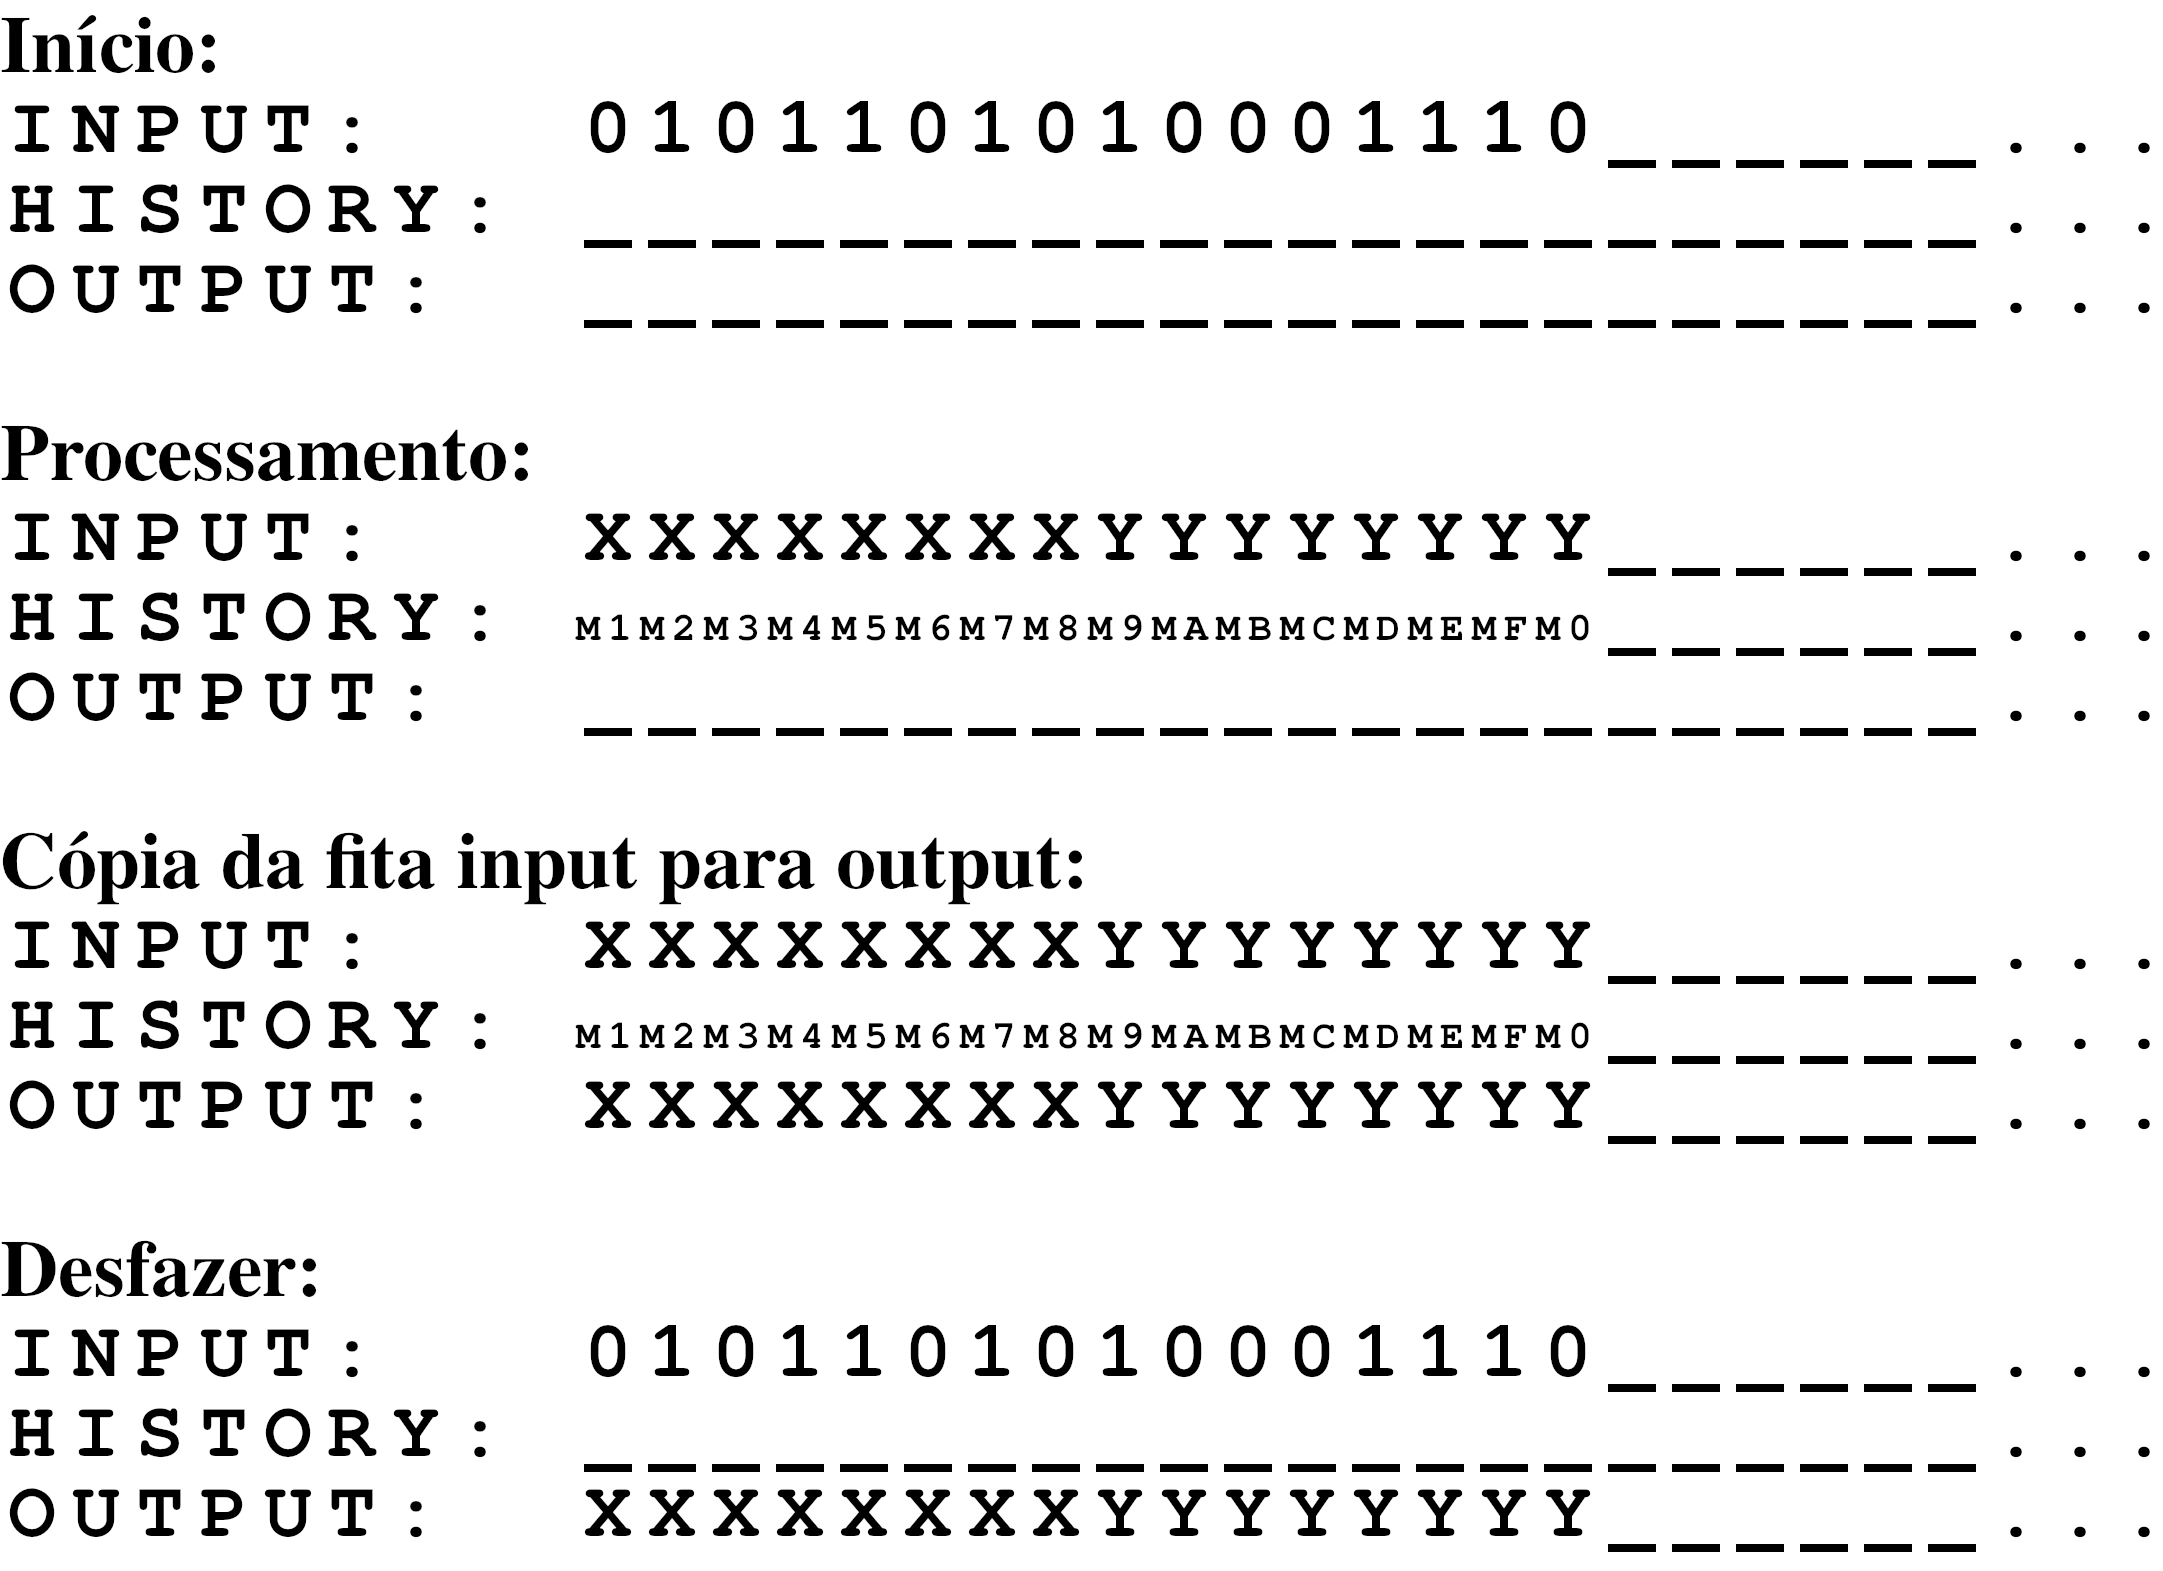
\includegraphics[width=0.9\linewidth]{bennett_machine.png}
\caption{Três etapas da máquina reversível de Bennett}
\label{fig:reversibility}
\end{figure}

Como ilustrado na Figura~\ref{fig:reversibility}, na primeira etapa, a máquina simula passo a passo a execução de uma máquina de Turing convencional, mas registra, na fita de histórico, o índice da regra aplicada em cada transição. Isso garante que todas as decisões possam ser revertidas posteriormente.

Na segunda etapa, o conteúdo da fita de trabalho é copiado para a fita de saída. Essa cópia é feita de forma reversível, sem registro no histórico, desde que a fita de destino esteja inicialmente em branco.

Na etapa final, a máquina reverte todas as transições da primeira etapa em ordem inversa, utilizando os dados da fita de histórico. Como a cópia da saída foi preservada, o resultado final permanece intacto. Ao término da operação, a fita de histórico retorna ao estado original (vazia), a de trabalho contém novamente a entrada, e a fita de saída apresenta o resultado da computação.

Formalmente, Bennett mostra que qualquer máquina de Turing padrão $S$ pode ser simulada por uma máquina reversível $R$. Se $S$ possui $f$ estados, $N$ quíntuplas e um alfabeto de $z$ símbolos, então $R$ terá $2f+2N+4$ estados, $4N+2z+3$ transições (quádruplas), e usará $u+1$, $u$ e $A+2$ quadrados em suas três fitas, onde $u$ é o número de passos da computação e $A$ o comprimento da saída.

\section{Discussão e otimização de espaço/tempo}

Um dos principais desafios da computação reversível é a necessidade de memória temporária para armazenar o histórico. Em computações longas, esse espaço cresce proporcionalmente ao número de passos. Para mitigar esse problema, Bennett propõe uma técnica de segmentação.

A ideia é dividir a computação em $n$ segmentos menores. Cada segmento executa parte da tarefa, salva um \emph{dump} com o estado final, e reverte suas operações, liberando espaço na fita de histórico antes de passar ao próximo segmento. O \emph{dump} atua como entrada para o segmento seguinte. Ao final, restam o resultado, a entrada original e os \emph{dumps} intermediários, que também podem ser apagados de forma reversível.

Para ilustrar, a Figura~\ref{fig:tradeoff} apresenta um gráfico do trade‑off entre o espaço de histórico e o número de segmentos.

\begin{figure}[ht]
\centering
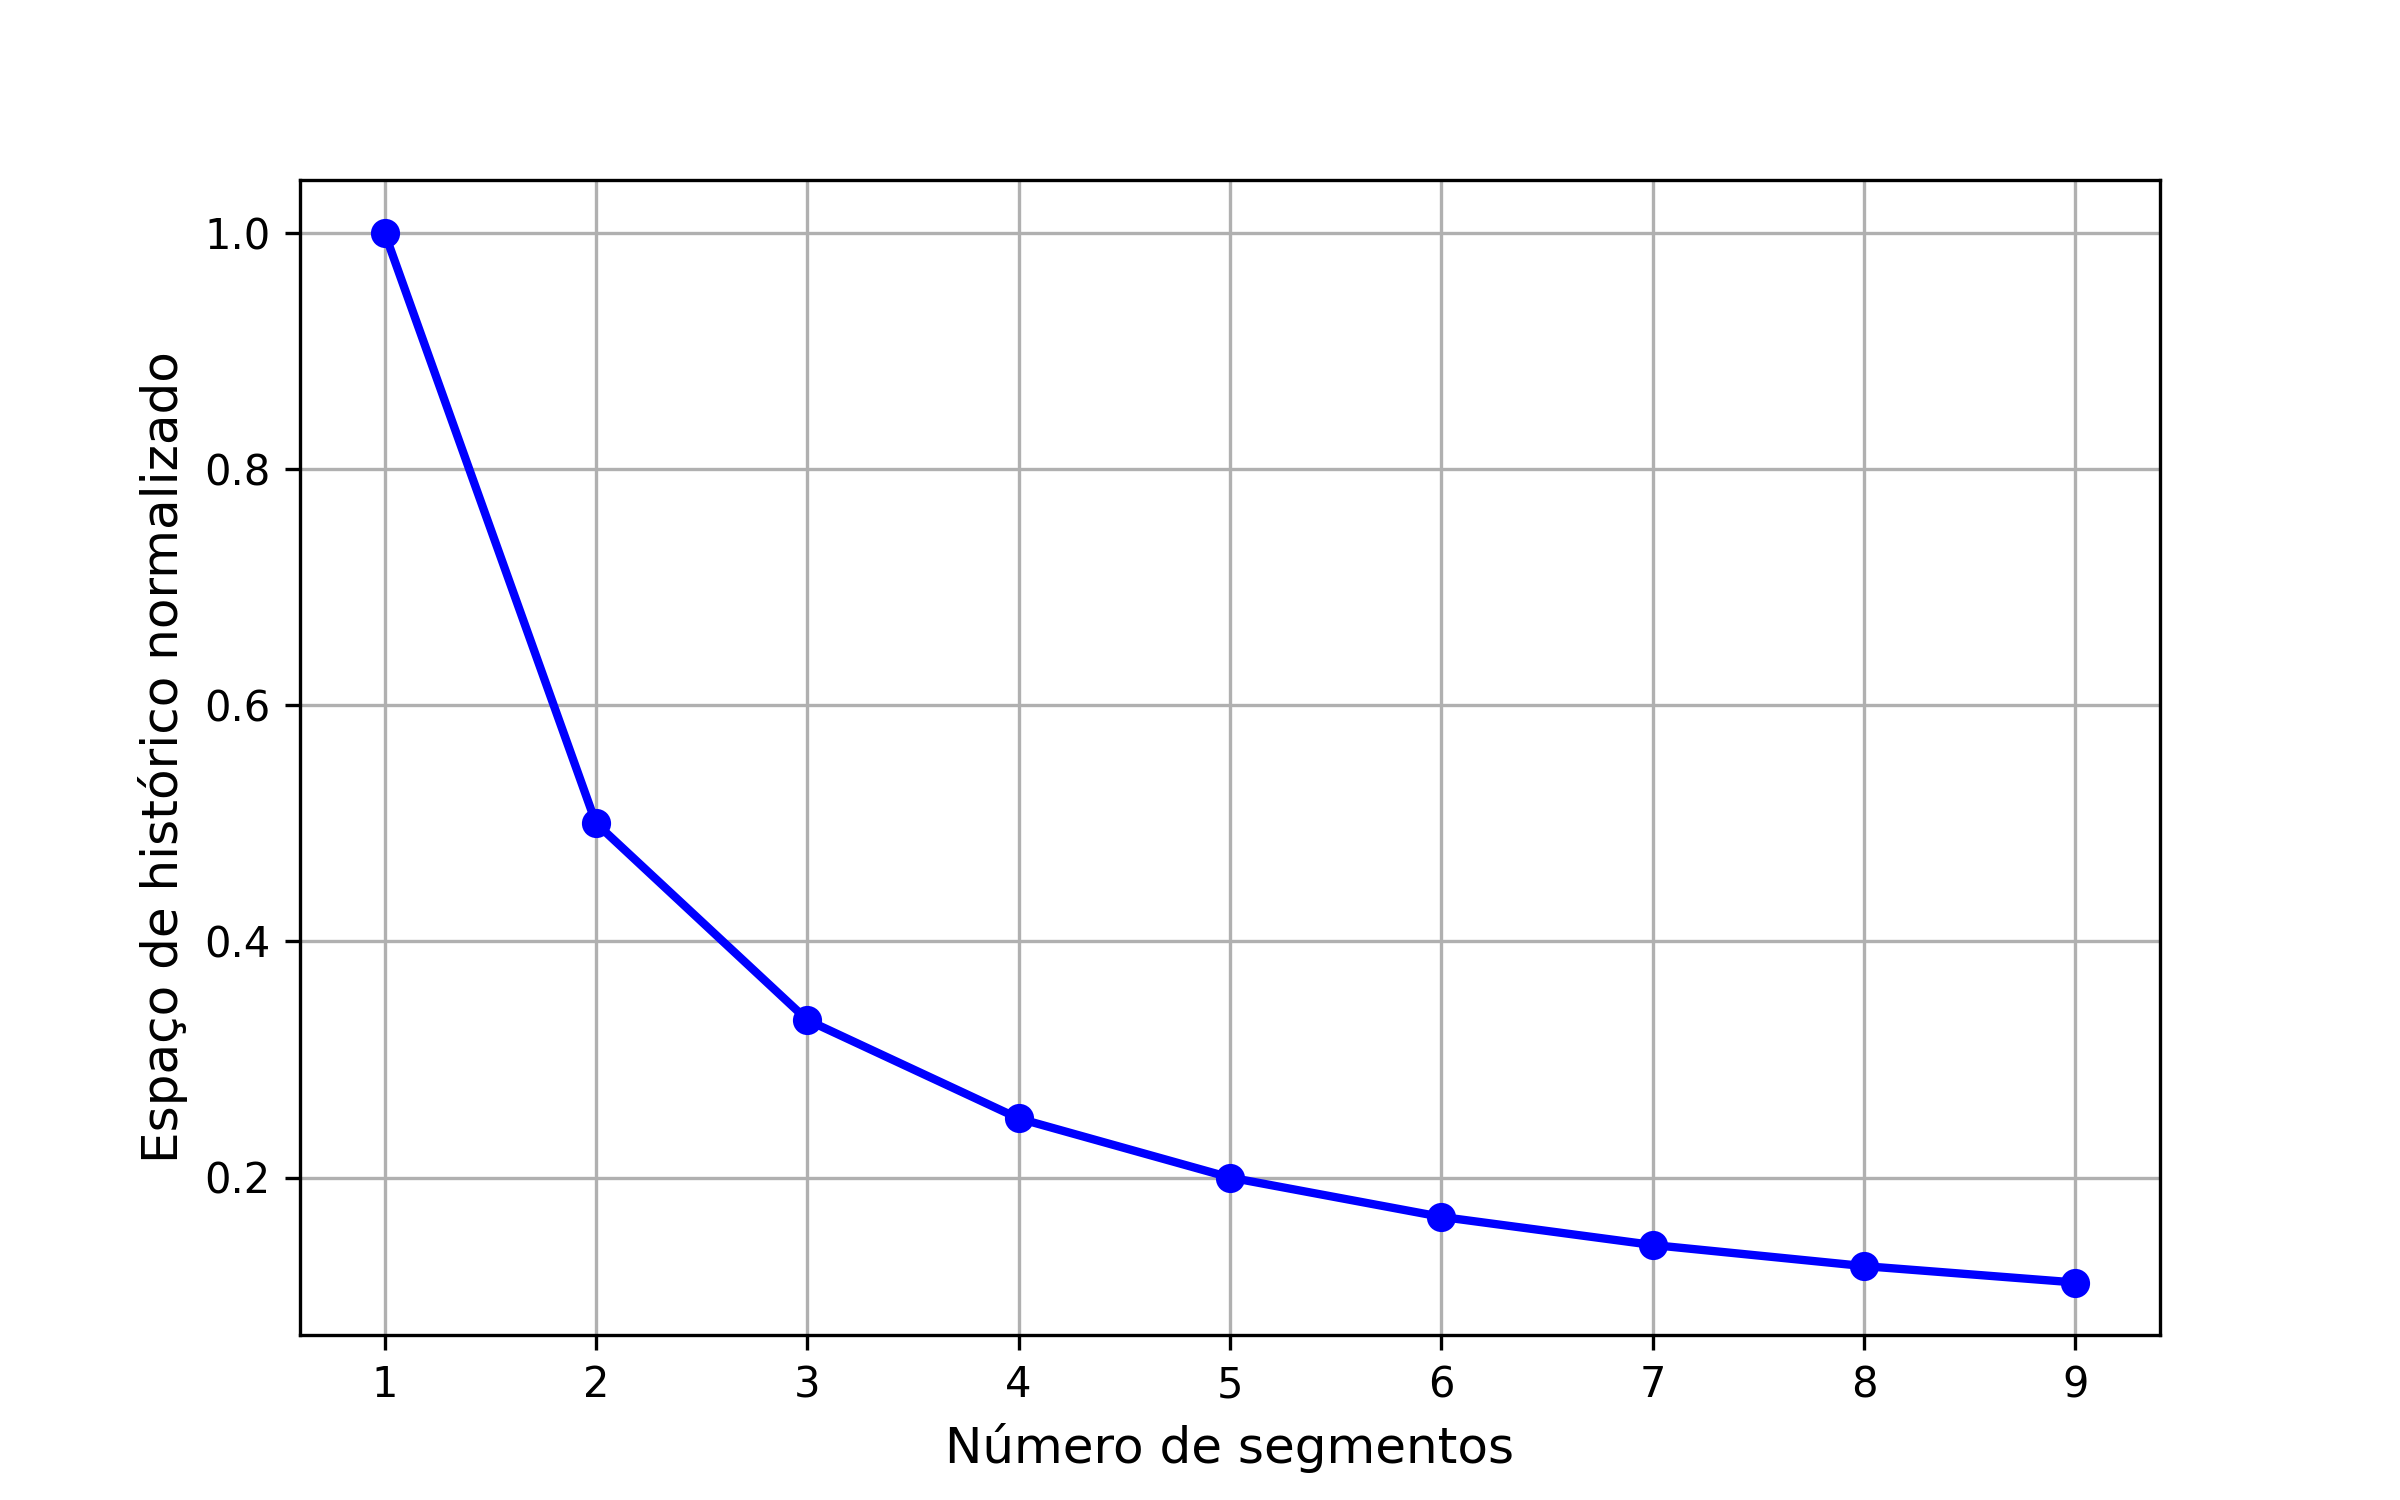
\includegraphics[width=1\linewidth]{space_time_tradeoff.png}
\caption{Trade‑off entre espaço de histórico e número de segmentos}
\label{fig:tradeoff}
\end{figure}

Com essa abordagem, o espaço temporário necessário é reduzido para aproximadamente $2s\sqrt{v}$, onde $s$ é o tamanho do \emph{dump} e $v$ o número total de passos. O tempo de execução aumenta modestamente. Para computações muito longas, a técnica pode ser aplicada de forma hierárquica, resultando em um crescimento de memória proporcional a $\log v$, mantendo a reversibilidade lógica e eficiência energética.

\section{Implicações físicas e bioquímicas}

A possibilidade de realizar computações logicamente reversíveis abre caminho para computadores fisicamente reversíveis, capazes de operar próximos ao equilíbrio termodinâmico e dissipar energia arbitrariamente pequena por passo computacional.

A natureza fornece um exemplo claro desse princípio: a RNA polimerase, enzima responsável pela síntese de RNA mensageiro a partir de DNA. Esse processo é logicamente reversível, pois trata-se de uma cópia fiel da informação genética, e também termodinamicamente reversível, já que as reações envolvidas ocorrem com auxílio de enzimas e em equilíbrio químico controlado.

Quando as concentrações de reagentes são alteradas, a mesma enzima pode realizar a degradação do RNA, comparando-o com o DNA original - operação igualmente reversível. No entanto, em sistemas biológicos, o RNA é frequentemente degradado por enzimas como a polinucleotídeo fosforilase, que o destrói sem referência à fita de DNA. Essa operação é logicamente irreversível e exige dissipação adicional de energia - cerca de $kT\ln4$ por nucleotídeo - para evitar a síntese aleatória de sequências sem sentido.

Esse contraste ilustra o custo físico da irreversibilidade lógica e reforça o potencial dos sistemas reversíveis como alternativa promissora para computação de baixo consumo energético. O modelo proposto por Bennett, além de teórica e logicamente viável, aponta caminhos concretos para o desenvolvimento de tecnologias computacionais mais sustentáveis em termos termodinâmicos.

\section{Conclusão}

O trabalho de Bennett (1973) oferece uma resposta ao desafio termodinâmico levantado por Landauer, demonstrando que é possível construir modelos de computação logicamente reversíveis com sobrecarga moderada e aplicabilidade geral. A máquina de três fitas proposta por Bennett, estruturada em três fases — execução direta, cópia e desfazer —, mostra como evitar a dissipação mínima de energia associada à perda de informação, registrando e posteriormente apagando o histórico de forma reversível.

Além de estabelecer um modelo formal com estimativas rigorosas de estados, tempo e espaço, Bennett apresenta uma técnica de segmentação que permite reduzir significativamente o espaço temporário necessário. Sua argumentação se estende ao domínio físico, indicando a viabilidade de computadores termodinamicamente reversíveis. O exemplo da RNA polimerase reforça esse ponto, evidenciando que a reversibilidade lógica e física já ocorre em sistemas naturais com grande eficiência. O estudo consolida, assim, os fundamentos para uma computação que respeita as leis da lógica e os limites da termodinâmica.

\section*{Agradecimentos}
Os autores agradecem à professora Juliana Kaizer Vizzotto pela oportunidade de desenvolver este estudo no âmbito da disciplina.

\begin{thebibliography}{00}
\bibitem{b1} Bennett, C. H. (1973). Logical reversibility of computation. IBM journal of Research and Development, 17(6), 525-532.
\bibitem{b2} Landauer, R. (1961). Irreversibility and heat generation in the computing process. IBM journal of research and development, 5(3), 183-191.

\end{thebibliography}

\end{document}
